\begin{center}
    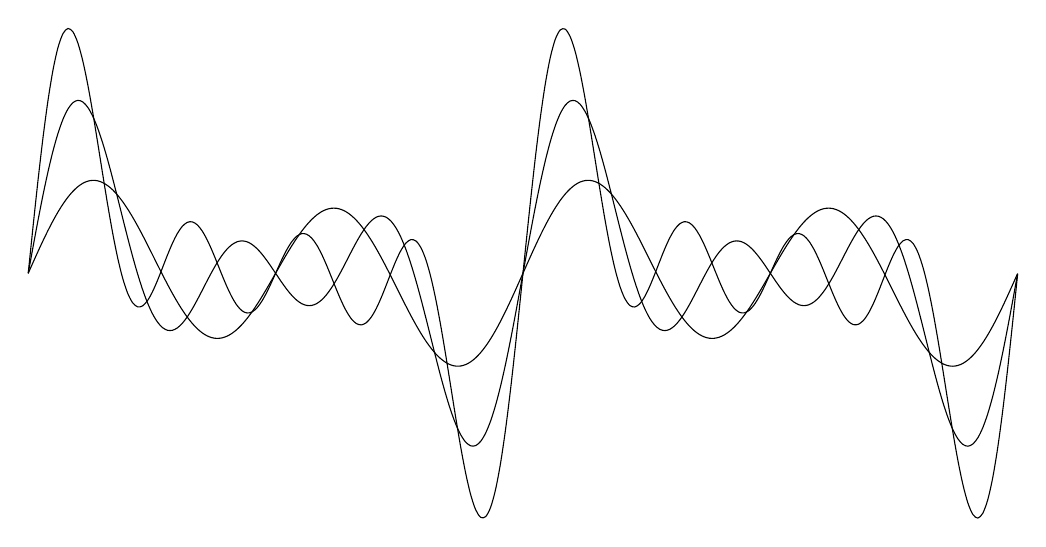
\begin{tikzpicture}
        % multiple sine cures with different frequencies and amplitudes between two points
            \draw[domain=0:4*pi, samples=200, smooth, variable=\x] plot ({\x}, {0.25*sin(deg(\x)) + sin(deg(2*\x))});
            \draw[domain=0:4*pi, samples=200, smooth, variable=\x] plot ({\x}, {0.5*sin(deg(\x)) + sin(deg(2*\x)) + sin(deg(3*\x))});
            \draw[domain=0:4*pi, samples=200, smooth, variable=\x] plot ({\x}, {0.75*sin(deg(\x)) + sin(deg(2*\x)) + sin(deg(3*\x)) + sin(deg(4*\x))});
            \tzcoor*(0, 0)(A)
            \tzcoor*(4*pi, 0)(B)
    \end{tikzpicture}
\end{center}


\begin{center}
    \begin{quote}
    \textit{A wave can be defined as a disturbance or variation that travels through a medium or space, transferring energy without permanently displacing the medium itself.}
    \end{quote}
\end{center}